\documentclass[11pt]{article}
\usepackage[utf8]{inputenc}
\usepackage{graphicx}
\usepackage{verbatim}
\usepackage{listings}
\usepackage{mathtools}
\lstset{language=C, frame=single}

\topmargin=-15mm
\oddsidemargin=0mm
\textwidth=159.2mm
\textheight=220mm

\title{Motion JPEG Encoding on Intel x86 using Streaming SIMD Extensions (SSE)}
\author{Paweł Kozłowski \and Łukasz Mazurek}


\begin{document}
\maketitle

\section{Introduction}
We have implemented 8 optimizations of \texttt{mjpeg\_encoder} program.
In the fig. \ref{times_plot} we can see time of encoding the movie\footnote{All time results used in this report are times of encoding \texttt{tractor.yuv} on \emph{Clinton} machine.} after each optimization.
All the optimizations together have reduced this time by factor 73.4, from 5475\,s to 74.6\,s.

\begin{figure}[h]
	\centering
	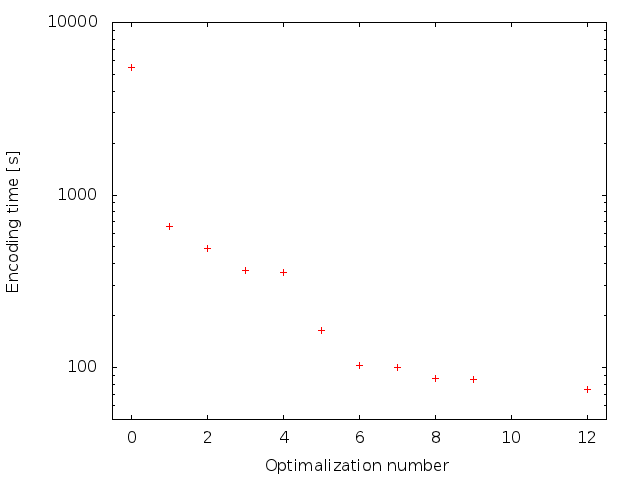
\includegraphics[width=0.7\textwidth]{img/times.png}
	\caption{Time of encoding \texttt{tractor.yuv} movie. After 8 optimizations this time was reduced from 5475\,s to 74.6\,s}
	\label{times_plot}
\end{figure}


\section{Optimalizations}
\subsection{Opt 1: Cosine array}
We recognized that first bottleneck (83.7\% of samples) is in this line:

\begin{lstlisting}
dct += coeff * (float) (cos((2*i+1)*u*PI/16.0f) 
     * cos((2*j+1)*v*PI/16.0f));
\end{lstlisting}
It contains slow computing of \emph{cos} function.
Since \texttt{i}, \texttt{u}, \texttt{j} and \texttt{v} are integers between 0 and 7, there are only 64 possible arguments of this \emph{cos}.
Therefore we can calculate the values of 
$$\cos \frac{(2a + 1) b \pi}{16}$$
once, for all $a, b \in \{0, \ldots, 7 \}$ and store them in array \texttt{cos\_table[8][8]}.
After that we can get the value of \emph{cos} function from the array instead of computing it every time.
Thus, considered line changed to:
\begin{lstlisting}
dct += coeff * cos_table[i][u] * cos_table[j][v];
\end{lstlisting}

Optimalization described above improved \texttt{mjpeg\_encoder} by factor 8.3, from 5475\,s to 657.8\,s.

\subsection{Opt 2: Products of cosines array}
Next observation: since there is only 64 possible values of $\cos$ function,
there is only $64 \cdot 64 = 4096$ possible values of product of two cosines.
Therefore we can store in array values of products
$$\cos \frac{(2a + 1) b \pi}{16}
\cos \frac{(2c + 1) d \pi}{16}$$
for all $a, b, c, d \in \{0, \ldots, 7 \}$.
Now considered line changed to:
\begin{lstlisting}
dct += coeff * cos_table[i][u][j][v];
\end{lstlisting}
This optimization improved program speed by factor 1.34, from 657.8\,s to 490.1\,s.

\subsection{Opt 3: SSE multiplying}
After first two optimizations the bottleneck was the floating-point addition and multiplication in following lines:
\begin{lstlisting}
float coeff = in_data[(y+j)*width+(x+i)] - 128.0f;
dct += coeff * cos_table[i][u][j][v];
\end{lstlisting}
Firstly, we changed these arithmetic operations from \texttt{float} to \texttt{int} operations, what improved program by factor 1.34, 
but finally we decided to come back to \texttt{float} numbers and change operations to \emph{SSE} addition and multiplication:
\begin{lstlisting}
__m128 coeff = _mm_load_ps(in_ptr);
__m128 cos_4float = _mm_load_ps(cos_ptr);

coeff = _mm_sub_ps(coeff, M128);
coeff = _mm_mul_ps(coeff, cos_4float);
_mm_store_ps(table, coeff);
dct += table[0] + table[1] + table[2] + table[3];

cos_ptr += 4;
in_ptr += 4;
\end{lstlisting}
Therefore we are doing 4 substractions at once and 4 multipications at once now.
This change improved the code 3 times, from 490\,s to 164\,s.

The problem was that \texttt{in\_data} was the type of \texttt{uint8\_t}
and was multiplied by \texttt{float} cosine.
At first we implemented a trick with casting \texttt{uint8\_t} pointer
to \texttt{\_\_m64} pointer and then converting it to float:
\begin{lstlisting}
__m128 coeff = _mm_cvtpu8_ps(*((__m64 *) in_ptr));
\end{lstlisting}
Unfortunately, this trick didn't work on \emph{Clinton} machine, 
since \texttt{\_\_m64} type is no longer supported on 64-bit machines.
Therefore we decided to change the type of \texttt{in\_data} to \texttt{float}.

\subsection{Opt 4: Dot product}
The next bottleneck was an addition of 4 \texttt{float}s.
This \texttt{float}s were results of multiplication 4 consecutive elements
of \texttt{in\_data} array and cosine array.
\begin{lstlisting}
coeff = _mm_mul_ps(coeff, cos_4float);
_mm_store_ps(table, coeff);
dct += table[0] + table[1] + table[2] + table[3];
\end{lstlisting}
We can do multiplication of four pairs of floats and sum up the results
in one \emph{SSE} operation: \textbf{dot product}:
\begin{lstlisting}
coeff = _mm_dp_ps(coeff, cos_4float, 0xf1);
_mm_store_ss(table, coeff);
dct += table[0];
\end{lstlisting}
This optimization improved code by factor 1.6 to 103\,s total time.

\subsection{Opt 5: Load operation moved out from a loop}
We recognized that \texttt{\_mm\_load\_ps} operation of input data 
is performed $64 \cdot 16$ times for each block.
\begin{lstlisting}
__m128 coeff = _mm_load_ps(in_ptr);
\end{lstlisting}
Since there are only 16 different values of possible input data to load
in a certain block, we can load it once and store in 16 registers:
\begin{lstlisting}
__m128 c[16];
for (i = 0; i < 16; i += 2) {
    c[i] = _mm_load_ps(in_ptr);
    c[1+1] = _mm_load_ps(in_ptr + 4);
    in_ptr += width;
}
\end{lstlisting}
This optimization improved program only by factor 1.03.

\subsection{Opt 6: \texttt{floor()} function removed. 
\texttt{uint8\_t quantization} changed to \texttt{float quantization}}
The next bottleneck was in the following line:
\begin{lstlisting}
out_data[(y+v)*width+(x+u)] = 
  (int16_t)(floor(0.5f + dct / (float)(quantization[v*8+u])));
\end{lstlisting}
Of course \texttt{floor} operation before casting to \texttt{int16\_t}
is unnecessary here, so we can just remove it.
Other slow operation in this line is casting \texttt{uint8\_t quantization} array to \texttt{float}.
Since \texttt{quantization} is a constant array $8 \times 8$ we can store it
in memory as a \texttt{float} array and avoid this casting each time.
These two changes improved our encoder by factor 1.18.

\subsection{Opt 7: Cos + malloc}
TODO: Paweł

This optimization improved our code by factor 1.10, from 83.6\,s to 76.0\,s.


\subsection{Opt 8: Zmiana koncepcji?}
TODO: Paweł

This optimization improved our code by factor 1.02, from 76.0\,s to 74.5\,s.

\end{document}
